%%%%%%%%%%%%%%%%%%%%%%%%%%%%%%%%%%%%%%%%%%%%%%%%%%%%%%%%%%%%%%%%%%%%%%%%%%%%%%%%
\chapter{Разработка}
\label{chap:dev}

Этот раздел посвящен разработке алгоритма извлечения вопросно-ответных пар, который включает в себя следующие этапы:

\begin{itemize}
\item Предобработка данных;
\item Кластеризация обращений по тематикам;
\item Извлечение ВОП.
\end{itemize}

Далее дается краткое описание подхода в целом, затем детально описывается каждый из этапов.

%%%%%%%%%%%%%%%%%%%%%%%%%%%%%%%%%%%%%%%%%%%%%%%%%%%%%%%%%%%%%%%%%%%%%%%%%%%%%%%%
\section{Обзор этапов подхода}
\label{sec:overview}
%%%%%%%%%%%%%%%%%%%%%%%%%%%%%%%%%%%%%%%%%%%%%%%%%%%%%%%%%%%%%%%%%%%%%%%%%%%%%%%%

\textbf{Этап 1~--- предобработка данных}. На данном этапе происходит подготовка обращений к отображению в ЧЗВ. Сырые данные содержат много шума: HTML разметка, заголовки электронной почты (напрмиер, <<01 июля 2001 г., 10:10 пользователь ... написал:>>), приветствия, благодарности и так далее. Этот шум не имеет прямого отношения к проблемам пользователей, что приводит к формированию тем, не отражающих действительного содержания обращений, и заметно влияет на качество алгоритма в целом. 

К шуму также относятся фрагменты програмного кода, логи и трассировки стека. Для таких данных характерен часто повторяющийся, небольшой набор слов, что также ведет к формированию тем, описывающих програмный код или логи, а не пользовательсике проблемы.

Для повышения качества результирующих ВОП применяется ряд эвристик предобработки, которые значительно доработаны в сравнение со статьей~\cite{original}. При этом также фильтруются обращения, которые заведомо не могут содержать вопроса или ответа. 

\textbf{Этап 2~--- кластеризация обращений по тематикам}. Для определения кластеров связанных обращений (в дальнейшем~--- тем) используется скрытое размещение Дирихле. LDA описывает каждую тему как вероятностное распределение по набору всех слов и для каждого обращения определяет вероятностное распределение по темам. Затем каждому обращению сопоставляется тема с наибольшей вероятностью. Для каждой темы определяется мешок слов (bag-of-words), как совокупность слов всех документов, принадлежащих данной теме. 

\textit{Bag-of-words}~--- это представление документа в виде набора слов с учетом их частоты, без учета порядка следования.

Используется перплекися для приблизительного определения количества тем. Точного определения количества тем не требуется, поскольку этап 3 включает в себя удлаление расфокусированных тем. В конце данного этапа темы проходят через фильтр, с целью удаления незначимых с точки зрения ЧЗВ тем.

\textbf{Этап 3~--- формирование ВОП}. Для каждого комментария в рамках обращения считается метрика близости между текстом комментария и соответствующей темой. На основе этой метрики определяются хорошо сформулированные вопросы и релевантные ответы на них. Удаляются расфокусированные темы~--- темы, не отражающие ни одну из реальных тем анализируемых данных

На рисунке~\ref{fig:common_scheme} изображена общая схема алгоритма, включающая все описанные выше этапы, а также этап экспертной оценки.

\begin{figure}[tph!]
\centerline{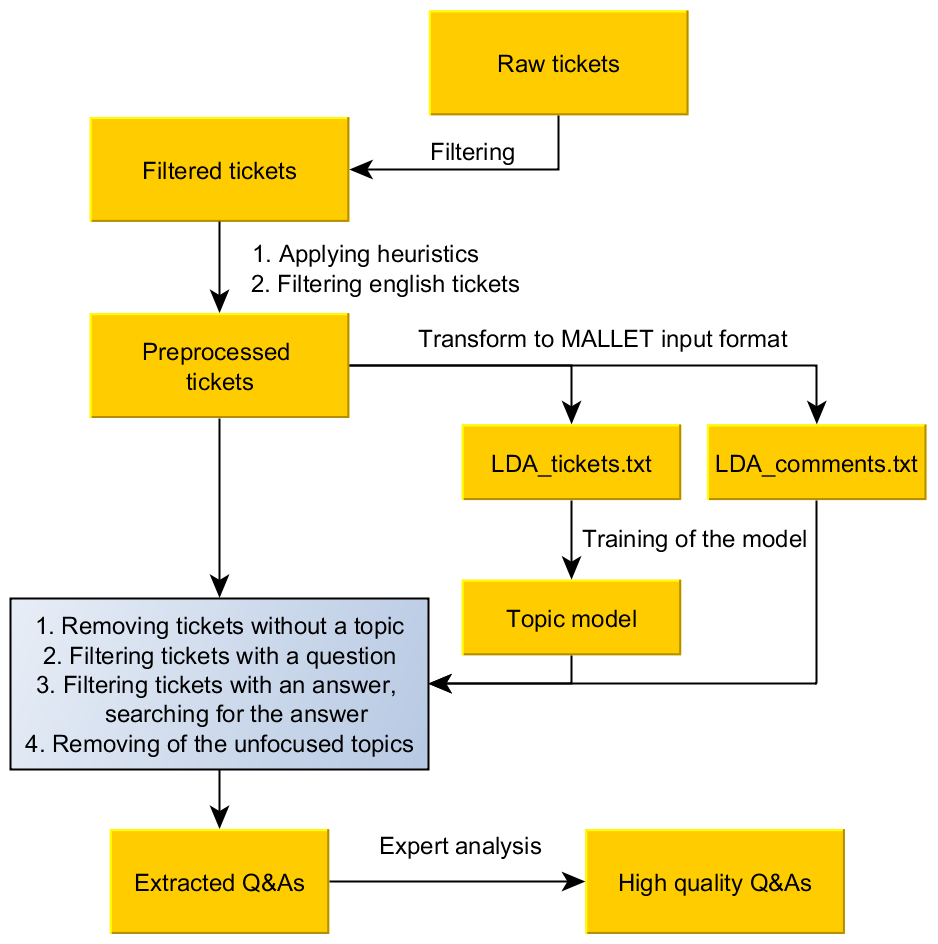
\includegraphics[width=11cm]{fig/schema2_eng.png}}
    \caption{Общая схема алгоритма}
    \label{fig:common_scheme}
\end{figure}

%%%%%%%%%%%%%%%%%%%%%%%%%%%%%%%%%%%%%%%%%%%%%%%%%%%%%%%%%%%%%%%%%%%%%%%%%%%%%%%%
\section{Предобработка данных}
\label{sec:dev}
%%%%%%%%%%%%%%%%%%%%%%%%%%%%%%%%%%%%%%%%%%%%%%%%%%%%%%%%%%%%%%%%%%%%%%%%%%%%%%%%

Исходные данные представляют собой 8500 обращений, собранных из различных каналов поступления обращений с помощью системы автоматизации запросов клиентов Zendesk. Каждое обращение содержат ряд метаданных. В то время как использование метаданных ограничивает область применения алгоритма, это позволяет повысить его качество. В данной работе использовалась метаинформация, широко распространенная для данных такого рода: статус обращения и авторство комментария.

Предполагается, что ответ на вопрос всегда содержится в одном комментарии, поэтому несколько комментариев не объединияются для создания ответа (секция~\ref{sec:features}). Для анализа использовались только обращения на английском языке.

Из входных данных были отфильтрованы обращения только со статусом "закрыто" и "выполнено". Данные статусы говорят о том, что обращения  имеют окончательный набор комментариев, в то время как другие обращения еще могут находиться в активном обсуждении.

Эвристики предобработки делятся на 2 категории: эвристики отображения и эвристики тематического моделирования. Первые предназначены для приведения обращений к виду, максимально близкому к виду ЧЗВ, вторые~--- применяются поверх первых и создают отдельное представление, используемое в LDA.

Для наглядности в таблице~\ref{comment_example} приведен простой пример необработанного комментария, полученного от пользователя через электронную почту, в таблице~\ref{heuristics_table} для данного примера можно увидеть результаты работы эвристик обоих типов.

\begin{table}[!ht]
\caption{Пример комментария}
\label{comment_example}
\centering
\begin{tabular}{|c}
\parbox[t]{8cm}{Hello JetBrains,~\\ 
I want to configure youtrack over SSL but
not able to find any solution or article on the subject. Could you help me?

~\\
Thanks in advance

~\\
Some Name~\\
Director / CEO~\\
+12 34 567890~\\
mail@companyname.com~\\
https://www.companyname.com/} \\
\end{tabular}
\end{table}

\subsection{Эвристики отображения}
\label{subsec:lnfheur}

\textit{Эвристика 1 (специфичные регулярные выражения): }  данная эвристика направлена на удаление фрагментов, зависящих от предметной области или используемого программного обеспечения. Например: информация, добавляемая системой управления обращениями; шаблоны оформления обращений через веб-форму, содержащие дополнительные поля (имя, e-mail, компания); и так далее. 

Регулярные выражение, соответствующие этой эвристике, а также другие, используемые в данной работе регулярыне выражения, представлены в приложении~\ref{appx01}.

\textit{Эвристика 2 (удаление цитат электронной почты):} 33\% обращений созданы через электронную почту. Комментарии в таких обращениях часто цитируют предыдущее сообщение. Как следствие, в тексте появляются дубликаты, которые приводят к искажению тематической модели. Механизм определения цитат, используемый Zendesk, не всегдя справляется со своей задачей. Каждый четвертый комментарий содержит цитату электроной почты. Для их удаления использовалась самостоятельно разработанная библиотека email-parser\footnote{https://github.com/JetBrains/email-parser}.

Библиотека email-parser позволяет удалять цитаты из электронных писем с точностью выше 97\% вне зависимости от используемого почтового клиента или языка пиьма. Библиотека разрабатывалась за рамками данного дипломного проекта, однако описаной делает её использование актуальным.

\textit{Эвристика 3 (удаление общих суффиксов):} большинство пользователей, как правило, имеют подпись, которая добавляется в конец каждого отправленного ими сообщения. Алгоритм для определения и удаляения таких подписей приводеится ниже (алгоритм~\ref{algo1}).

\vspace{\baselineskip}
\begin{algorithm}[H]
		\SetAlgoLined
		\KwData{commentsList - список комментариев}
		\KwResult{modifiedCommentsList - модифицированный список комментариев}
		$suffixLength \leftarrow$ инициализация массива длины $commentsList.size$ нулями;\\
		\For{$i\leftarrow 1$ \KwTo $commentsList.size$}{
			\For{$j\leftarrow 1$ \KwTo $commentsList.size$}{
				$suffix \leftarrow$ определить общий суффикс для $commentsList[i]$ и $commentsList[j]$\\
				\While{$suffix[1]$ не символ новой строки}{
					удалить первый символ $suffix$;\\
				}
				$update(suffix, i)$;\\
				$update(suffix, j)$;\\
			}	
		}
		\For{$i\leftarrow 1$ \KwTo $commentsList.size$}{
			удалить из $commentsList[i]$ последние $suffix[i]$ символов;\\
		}
		
		\Fn{update(suffix, x)}{
		\If{$suffix.length \ge suffixLength[x]$}{
					$suffixLength[x] \leftarrow suffix.length$;\\
				}}

	\caption{Удаление общих суффиксов}
	\label{algo1}
\end{algorithm}
\vspace{\baselineskip}

Для удаления таких подписей предлагается следующее:

 \begin{itemize}
\item Для всех комментариев в исходных данных попарно посчитать общий суффикс;
\item У каждого комментария удалить суффикс максимальной длины;
\end{itemize}

Суффикс определяется построчно, что позволяет избежать частичного удаления абзацев с полезной информацией.

\textit{Эвристика 4 (короткие абзацы):} многие сообщения начинаются со слов приветствия и заканчиваются словами благодарности (рисунок~\ref{fig:zdesk_ticket}, таблица~\ref{comment_example}). Как правило, эти фрагменты выделены в отдельные абзацы (отделены символом новой строки) и значительно короче основной части сообщения (20-25 символов против 300-500). Данная эвристика удаляет (при наличии) один короткий начальный абзац и все короткие конечные абзацы. Абзац является коротким, если он состоит из 3 или меньше слов. Это число было определено эмпирически. Дополнительно этот шаг позволяет удалить фрагменты подписи, оставшиеся после эвристики 3.

Подписи в основном состоят из нескольких коротких строк (таблица~\ref{comment_example}), которые в большинстве случаев попадают под данную эвристику. Поэтому для последних строчек текста данную эвристику имеет смысл применять многократно. С другой стороны, приветствие встречается в начале текста не более одного раза. Поэтому здесь эвристика применяется один раз во избежание удаления полезной информации.

\begin{table}[!ht]
\caption{Эффект применения эвристик}
\label{heuristics_table}
\centering
\begin{tabular}{|c|c|}
\hline
Версия для ЧЗВ & Версия для LDA \\
\hline
\parbox[t]{4cm}{I want to configure youtrack over SSL but
not able to find any solution or article on the subject} & \parbox[t]{4cm}{configure SSL solution article subject}\\
\hline
\end{tabular}
\end{table}

\textit{Эвристика 5 (частые предложения):} данная эвристика была взята из статьи~\cite{original} и говорит о том, что предложения, встречающиеся на всем наборе обращений более 15 раз, не содержат информации, специфичной для конкретного вопроса. К таким фразам могут относиться: <<Моя проблема заключается в следующем>>, <<Благодарим вас за обращение>> и так далее.

Стоит отметить, что учет предложений, состоящих из одного слова, или игнорирование регистра текста приводит к частичному удалению предложений и, как следствие, ухудшению внешнего вида ВОП.

Как результат применения описанных выше эвристик, текст комментариев часто может начинаться с нижнего регистра (ввиду удаления приветствий) и содержать лишние пустые строки, что снижает читаемость. Данные недостатки следует исправить, так как именно в таком виде ВОП будут показываться экспертам. Для этого необходимо удалить пустые строки и лишние пробелы, а также перевести первый непробельный символ в верхний регистр.

\subsection{Эвристики тематического моделирования}
\label{subsec:ldaheur}

Эвристики из данной группы применяются с целью повышения качества LDA. Поскольку при этом теряется часть информации, необходимой для отображения ЧЗВ, необходимо сохранять две версии для каждого из комментариев, как показано в таблице \ref{heuristics_table}.

\textit{Эвристика 6 (удаление пользовательских данных):} пользовательские данные ухудшают качество LDA. Например, тема, включающая в себя имя некоторого пользователя, будет содержать обращения, в которых часто встречается это имя, несмотря на то, что сами обращения могут относиться к разным подсистемам программного продукта и, соответственно, иметь различные темы. 

На этом этапе предлагается удалять такие фрагменты текста, как: унифицированные идентификаторы ресурса (URI), пути в файловой системе, адреса электронной почты, названия сайтов (www.mysite.com) и некоторые другие (приложение~\ref{appx01}).

\nomenclature{URI}{Uniform Resource Identifier, унифицированый идентификатор ресурса}

\textit{Эвристика 7 (удаление длинных абзацов):} абзацы естественной речи для ИТ-дискуссий редко превышают 800 символов, в то время как длина машинно сгенерированного текста (логи, трассировки, код) часто больше этого значения.

Данная эвристика является особенно важной, поскольку именно большие объемы терминологически бедного машинно сгенерированного текста оказывают наиболее заметное негативное влияние на тематическу модель.

\textit{Эвристика 8 (абзацы с пунктуацией):} необходима для определения коротких (менее 800 символов) фрагментов машиино сгенерированно текста. Было установлено, что абзацы длиной больше 200 символов и содержащие более 6\% символов пунктуации также являются машинно сгенерированными. В качестве символов пунктуации использовался следующий набор символов:

\vspace{\baselineskip}
\noindent \textit{'`-=|\/*+,;:()\{\}[]<>\%\$@\&\_}
\vspace{\baselineskip}

Ограничение на минимальную длину абзаца позволяет избежать ложных срабатываний. Это также позволяет сохранить, например, название ошибки или полное имя класса.

\textit{Эвристика 9 (удаление стоп-слов):} предназначена для удаления наиболее частых слов английского языка, которые не помогают в определении темы в виду своего общего назначения. 

Данная задача решается средствами библиотеки MALLET~\cite{MALLET}. Библиотека MALLET используется для решения задач тематического моделирования (секция~\ref{subsec:lda}) и предоставляет набор предопределенных функций для модификации данных перед построением тематической модели. Одна из такий функций позволяет удалить наиболее распространенные английские слова (стоп-слова).

К ним стоит добавить слова, часто используемые в анализируемой области ('java' или 'class' для обсуждения разработки на Java).В рамках выбранной предметной области такие слова также являются стоп-словами и затрудняют определение тем.

\subsection{Фильтрация обращений}
\label{subsec:ticketfilter}

После применения эвристик некоторые из комментариев могут оказаться пустыми, в то время как другие могут не содержать ответа от технического специалиста. Из таких обращений не удастся извлечь ВОП. Воспользуемся метаинформацией об авторстве и отфильтруем обращения, имеющие не пустой первый комментарий (в версии для LDA) и не менее одного не пустого комментария от сотрудника технической поддержки.

Обращения, содержащие длинную нить обсуждения (более 6 комментариев), вероятно, имеют одну из следующих проблем: вопрос плохо сформулирован, вопрос слишком специфичен, ответ недостаточно полон и содержится в нескольких комментариях. Поскольку мы считаем, что ответ всегда содержится в не более чем одном комментарии (секция~\ref{sec:features}), корректную ВОП в данном случае составить не удасться. Такие обращения не имеют ценности с точки зречия ЧЗВ, их необходимо удалить.

Спицифичные для предметной области обращения, например: обращение закрытое по причине слияния с другим обращением, и так далее~--- также подлежат удалению.

%%%%%%%%%%%%%%%%%%%%%%%%%%%%%%%%%%%%%%%%%%%%%%%%%%%%%%%%%%%%%%%%%%%%%%%%%%%%%%%%
\section{Тематическое моделирование}
\label{sec:topicmodeling}
%%%%%%%%%%%%%%%%%%%%%%%%%%%%%%%%%%%%%%%%%%%%%%%%%%%%%%%%%%%%%%%%%%%%%%%%%%%%%%%%

Тематическое моделирование~\cite{TM} позволяет (а) сгруппировать схожие обращения по темам (например, одна тема может касаться почтовой интеграции, а другая~--- вопросов о продлении подписки для пользователей), (б) охарактеризовать каждую тему списком терминов~--- мешком слов (\mbox{bag-of-words}).

\subsection{Скрытое размещение Дирихле}
\label{subsec:lda}

В работе использовался метод скрытого размещения Дирихле и его реализация на Java~\cite{MALLET}. LDA работает с любыми текстовыми документами, поэтому далее будет использоваться термин 'документ' для описания обращения, как совокупности его комментариев.

LDA~--- это вероятностная тематическая модель, не требующая размеченных данных для обучения, однако требующая указания количества моделируемых тем. LDA описывает каждую тему $t$, как вероятностное распределение по всем словам из входных данных ($\phi_t$). Каждый документ $d$ описывается вероятностным распределением по темам ($\theta_d$). Более подробно LDA описывается в секции~\ref{ch1:lda}.

Распределения $\phi$ и $\theta$ в свою очередь зависят от гиперпараметров $\alpha$ и $\beta$ соответственно. Реализация LDA в~\cite{MALLET} поддерживает автоматическую оптимизацию этих параметров с использованием сэмплирования по Гиббсу~\cite{gibbs}. Программисту остается лишь указать количество тем.

Определение количества тем~--- нетривиальная задача, которая не рассматривается в оригинальной статье. В данной работе для этой цели предлагается использовать \textit{меру неупорядоченности} (perplexity, перплексия)~\cite{LDA}.  Эта метрика показывает сходство между терминами документов и их темой (меньше~-- лучше), но не отражает семантическую связь. Другими словами, при оценивании тематической модели учитывается частота появления слов в документах, но при этом нет возможности учесть насколько некоторая пара слов близка по смыслу между собой. Поэтому так важен этап экспертной оценки.

Тем не менее перплексия позволяет определить минимальное число тем, при котором обращения начинают разделяться на четко выраженные подтемы. Критерием является значительное замедление скорости падения перплексии с ростом числа тем. В секции~\ref{subsec:deleteunfocusedtopics} показывается как можно избавиться от расфокусированных тем, поэтому точное определение количества тем не требуется. Основываясь на перплексии, для построения тематической модели было выбрано количество тем, равное 200 (рисунок~\ref{fig:perpl}). Существуют другие подходы к определению оптимального количества тем. Например, в статье~\cite{TMuse} для данной задачи используется подход, основанный на генетических алгоритмах.

\begin{figure}[tph!]
\centerline{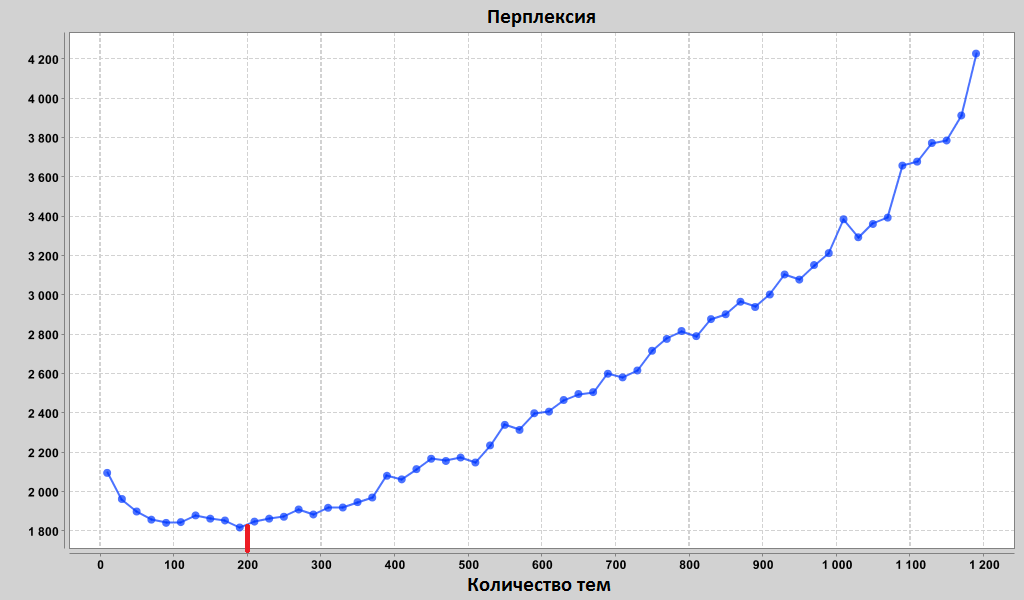
\includegraphics[width=11cm]{fig/perpl.png}}
    \caption{Зависимость перплексии от числа тем}
    \label{fig:perpl}
\end{figure}

В результате тематического моделирования для каждого документа определяется вероятностное распределение по темам $\theta_{d,t}$. Мы сопоставляем каждому обращению одну тему~--- тему с максимальной вероятностью. Однако, если для обращения $d$ вероятность каждой темы $\theta_{d,t}<0.25$, то такое обращение не имеет четко выраженной темы и для него не будет определяться ВОП.

Мешок слов каждой темы определяется, как совокупность слов всех документов, принадлежащих данной теме.

Способ построения тематической модели аналогичен предлагаемому в~\cite{original}. Дополнительно применяется перплексия для приблизительного определения количества тем.

%%%%%%%%%%%%%%%%%%%%%%%%%%%%%%%%%%%%%%%%%%%%%%%%%%%%%%%%%%%%%%%%%%%%%%%%%%%%%%%%
\section{Формирование пар вопрос-ответ}
\label{sec:qaforming}

Процесс получения ЧЗВ из смоделированных тем состоит из трех шагов: фильтрация неинформативных тем, определение пар вопрос-ответ, удаление расфокусированных тем. Первый шаг является новым, в то время как другие два~--- взяты из опорной статьи~\cite{original} за исключанием пороговых значений.

\subsection{Дополнительная фильтрация}
\label{subsec:topicfilter}

Данный этап не обязателен и предполагает некоторые априорные знания о данных, а также то, что алгоритм уже запускался ранее. Используемые в работе данные (обращения в техническую поддержку) могут содержать большое количество типичных, повторяющихся обращений с шаблонными ответами (просьбы о сбросе пароля; вопросы о недоступности сервиса и так далее). Такие обращения являются частыми, но не несут полезной информации для ЧЗВ.

После построения тематической модели можно найти мешки слов для таких тем. Следует запомнить 10 наиболее значимых слов для каждой из них (топ-10 слов). При последующих запусках LDA удаляются темы, для которых выполняется условие: хотя бы половина из топ-10 слов темы совпадают с одной из фильтруемых тем. Темы проверяются на частичное совпадение, поскольку LDA недетерминирован и мешки слов могут незначительно отличаться от запуска к запуску.

Данный фильтр позволяет избавиться от шаблонных ВОП, но может негативно влиять на метрики качества (раздел \ref{chap:quality}), поскольку удаляемые таким образом темы четко выражены и содержат большое количество обращений.

\subsection{Определение вопросов и ответов}
\label{subsec:findqa}

Для определения вопросов и ответов для каждого комментария вычисляется метрика близости с соответствующей темой. Для этого использовалось косинусное расстояние~\cite{cosine}: 
$$
\cos(e, t)=\frac{\sum_{i=1}^nt_ie_i}{\sum_{i=1}^n(t_i)^2\sum_{i=1}^n(e_i)^2}\eqno(7)
$$
где $t$~--- вектор, соответствущий мешку слов темы, $e$~--- вектор, соответствующий словам комментария в представлении для LDA. Чем больше значение косинуса, тем сильнее комментарий связан с темой.

Пример получения векторов для текстов приведен в таблице~\ref{text_vect}. Пусть имеется два текста~--- $t$ и $e$:

\begin{itemize*}
\item t: some short text text
\item e: some another text
\end{itemize*}

\begin{table}[!ht]
\caption{Пример построения векторов}
\label{text_vect}
\centering
\begin{tabular}{|c|c|c|c|c|c|}
\hline
 & some & short & another & text \\
\hline
t & 1 & 1 & 0 & 2\\
\hline
e & 1 & 0 & 1 & 1\\
\hline
\end{tabular}
\end{table}

Для каждого из слов (для обоих текстов) считается сколько раз оно появилось в каждом из текстов. На основе данных значений строятся соответсвующие векторы.

Комментарий выбирается в качестве \textit{вопроса} при выполнении трех условий: (a) это первый комментарий в обращении; (б) косинус комментария и темы ($\cos(Q,T)$) выше порога 0.15; (в) длина комментария не превышает 1000 символов (более длинный текст комментария говорит о слишком специфичном для конкретного пользователя вопросе).

Условия выбора комментария в качестве \textit{ответа}: (а) это не первый комментарий в обращении; (б) не является комментарием инициатора обращения; (в) косинусное расстояние с темой ($\cos(A,T)$) выше порога 0.15 и максимально среди других кандитатов на ответ.

Обращения в службу поддержки, типично представляют собой диалог с итеративным уточнением деталей, предоставлением дополнительной информации и попытками дать окончательный ответ. В качестве вопроса выбирается только инициирующий комментарий, поскольку все последующие комментарии пользователя не будут содержать полной информации о проблеме. Ответом считается комментарий сотрудника технической поддержки, наиболее совпадающий с темой по используемым терминам. Таким образом, обеспечивается сходство терминологии между вопросом и ответом для найденных ВОП.

\subsection{Удаление расфокусированных тем}
\label{subsec:deleteunfocusedtopics}

Ввиду отсутствия возможности точно определить моделируемое число тем (секция~\ref{sec:topicmodeling}) возможны случаи, когда реальное количество тем будет меньше или больше смоделированного. В первом случае полученные после LDA темы будут слишком общими, что приведет к большим различиям между терминологий темы и принадлежащими ей обращениями и, как следствие, пониженному количеству и качеству найденных ВОП. Во втором~--- создадутся фантомные темы, терминология которых будет плохо совпадать с реальными данными. Удалим такие расфокусированные темы за счет введения минимальной доли ВОП (8) со значением 0,1.
$$
\frac{|QAPairs_t|}{|tickets_t|}>threshold\eqno(8)
$$
где $|QAPairs_t|$~--- количество ВОП, извлеченных из обращений, принадлежащих к теме $t$; $|tickets_t|$~--- количество обращений, принадлежащих к теме $t$, $threshold$~--- минимальная доля ВОП.

Образованные ВОП упорядочиваются (в рамках каждой темы или глобально) с использованием гармонического среднего между $\cos(Q,T)$ и $\cos(A,T)$. Гармоническое среднее (9) для получения высокого значения требует, чтобы все составляющие были высоки, таким образом, гарантируется, что и вопрос, и ответ имеют высокое качество.
$$
H = \frac{n}{\sum_{i=1}^n\frac{1}{x_i}}\eqno(9)
$$
После этого ВОП передаются эксперту для валидации и редактирования перед публикацией.  Данный этап описывается в разделе~\ref{chap:quality}.

\section{Вывод}
\label{sec:dev_concl}

В данном разделе представлен алгоритм извлечения вопросно-ответных пар. Описаны основные составляющие этапы, такие как:

\begin{itemize*}
\item Предобработка данных;
\item Кластеризация обращений по тематикам;
\item Извлечение ВОП.
\end{itemize*}

Рассмотрены раличные типы эвристик предобработки данных; обоснована необходимость фильтрации данных. А также описаны способы определения количества тем и удаления расфокусированных тем, определены условия, которым должны удовлетворять найденные вопросно-ответные пары.